% BEGIN_FOLD
\documentclass[a4paper,11pt]{report} 
\usepackage[english]{babel} 
\usepackage[utf8]{inputenc}	
\usepackage{graphicx} 	   	
\usepackage{float}	 	
\usepackage[font=small, font=it, labelfont=bf]{caption} 
\usepackage[font=small, font=it, labelfont=bf]{subcaption} 	
\usepackage{comment} 		
\usepackage{hyperref} 		
\usepackage{url}
\usepackage{printlen}

\pagestyle{plain} 

% END_FOLD


\begin{document}
	
\chapter{Python Figures}

In the next chapter, python figures will be shown. \\
The text width of this document is \uselengthunit{cm}\printlength{\textwidth}

\section{The python figures}

In this section python figures are shown. Use this text for font size comparison. Note, that this is for 11pt report class. 

\begin{figure}
	\centering
	\begin{subfigure}{0.49\textwidth}
		\centering
		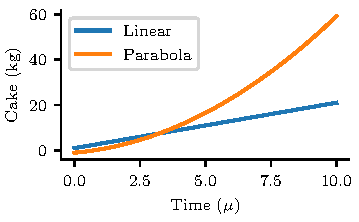
\includegraphics[width=1\linewidth]{fig/TwoGolden.pdf}
		\caption{}
	\end{subfigure}
	\begin{subfigure}{0.49\textwidth}
		\centering
		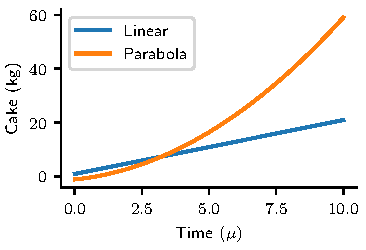
\includegraphics[width=1\linewidth]{fig/TwoInnerGolden.pdf}
		\caption{}
	\end{subfigure}
	\caption{8pt and $8$ pt with golden ratio of inner figure.}
\end{figure}

\begin{figure}
	\centering
	\begin{subfigure}{0.49\textwidth}
		\centering
		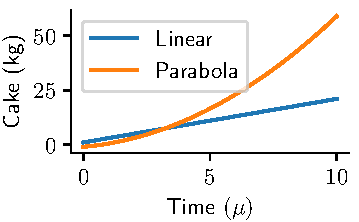
\includegraphics[width=1\linewidth]{fig/TwoGolden11.pdf}
		\caption{}
	\end{subfigure}
	\begin{subfigure}{0.49\textwidth}
		\centering
		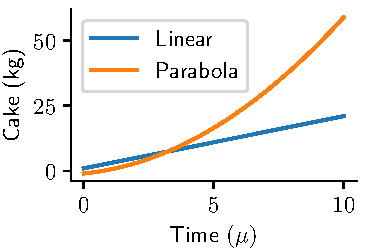
\includegraphics[width=1\linewidth]{fig/TwoInnerGolden11.pdf}
		\caption{}
	\end{subfigure}
	\caption{10pt and 10 pt with golden ratio of inner figure}
\end{figure}

\begin{figure}
\centering
\begin{subfigure}{0.8\textwidth}
	\centering
	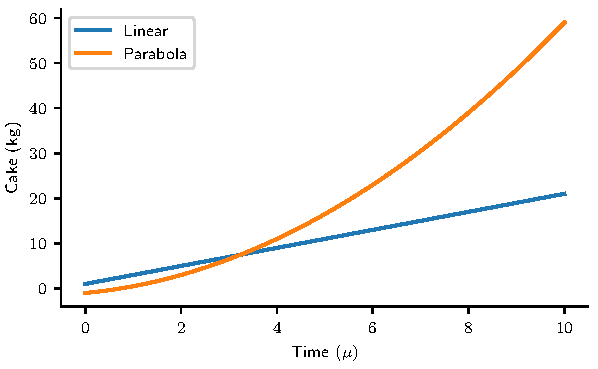
\includegraphics[width=1\linewidth]{fig/OneGoldenSmall.pdf}
\end{subfigure}
\caption{8 pt 0.8 size text width}
\end{figure}

\begin{figure}
\centering
\begin{subfigure}{0.99\textwidth}
	\centering
	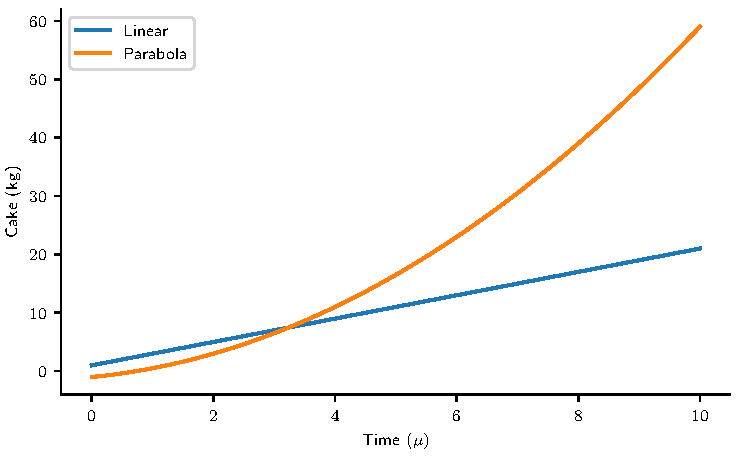
\includegraphics[width=1\linewidth]{fig/OneGoldenFull.pdf}
\end{subfigure}
\caption{8pt full width}
\end{figure}

\end{document}